\documentclass{beamer}

\usecolortheme[light]{solarized}

\beamertemplatenavigationsymbolsempty


\usepackage{booktabs}
\usepackage{graphicx}
\usepackage{hyperref}
\usepackage{minted}
\usepackage{moresize}
\usepackage{standalone}
\usepackage{tcolorbox}
\usepackage{tikz}
\usepackage[normalem]{ulem}
\usepackage{xpatch}
\usepackage{fix-cm}

\xpatchcmd{\sout}
  {\bgroup}
    {\bgroup\def\ULthickness{2pt}}
      {}{}

\usetikzlibrary{calc, patterns}

\definecolor{twitter}{RGB}{64, 153, 255}
\definecolor{github}{RGB}{211, 211, 211}

\newcommand{\assetsfolder}{./assets}
\newcommand{\revisitresearchfolder}{$HOME/rsc/revisiting-axelrod-second}
\newcommand{\moranresearchfolder}{$HOME/rsc/axelrod-moran}
\newcommand{\mlresearchfolder}{$HOME/rsc/ml-paper}

\begin{document}

    \begin{frame}
        \begin{center}
            \Huge
                Reproducible Science
                Reinforcement Learning
                Evolution

               \vfill

            \Large
               Vince: \href{https://twitter.com/drvinceknight}{@drvinceknight}\\
        \end{center}

        % Thank you very much ...  My name is Vince Knight and it's a true pleasure
        % to be speaking here today. Thank you to Marc Harper for the
        % invitation. I'll be speaking to you today about 3 topics that are
        % linked.
    \end{frame}

    \begin{frame}
               \begin{columns}
                   \begin{column}{.45\textwidth}
                       \begin{center}
                       
\includegraphics[height=3cm]{\assetsfolder/CUident_CMYK.eps}
                       \end{center}

                       \begin{center}
                       
\includegraphics[height=3cm]{\assetsfolder/axelrod_logo.png}
                       \end{center}
                   \end{column}
                   \begin{column}{.45\textwidth}
                       \begin{center}
                       
\includegraphics[height=3cm]{\assetsfolder/ssi-logo.png}
                       \end{center}

                       \pause
                       \begin{center}
                       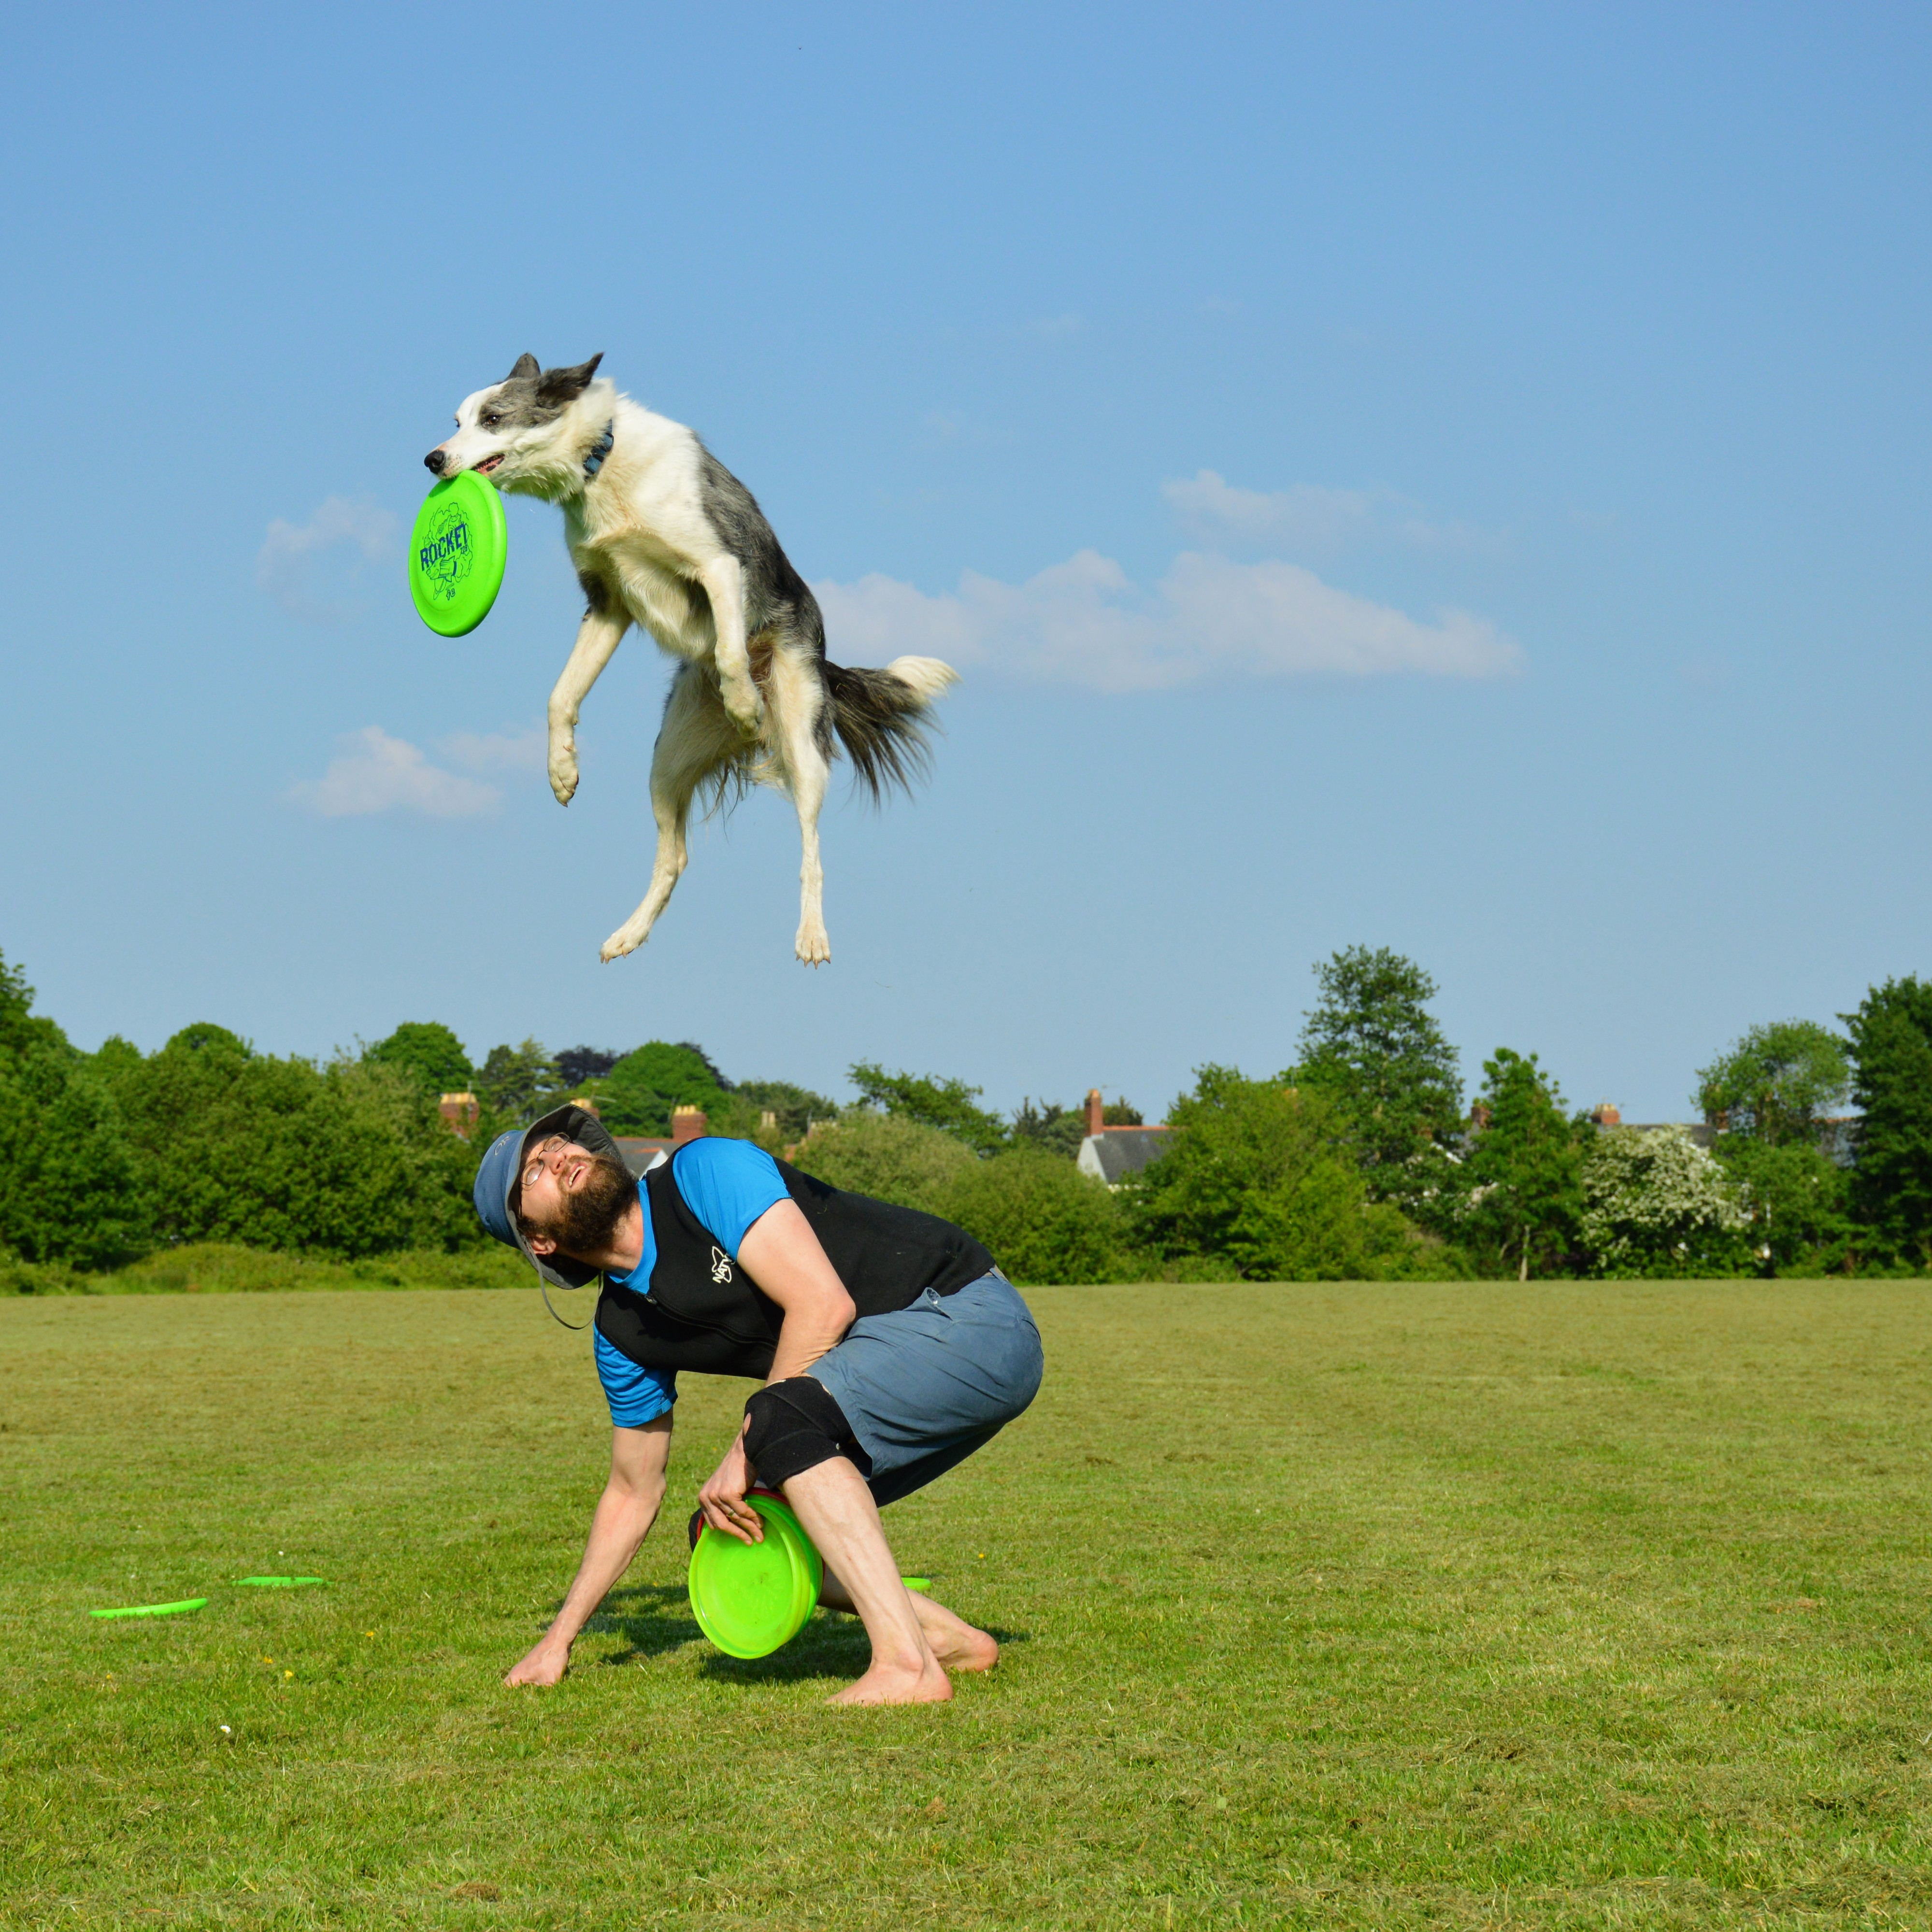
\includegraphics[height=3cm]{\assetsfolder/flying_dog.jpg}
                       \end{center}
                   \end{column}
               \end{columns}

        % Notes I am an associate professor at Cardiff University's School of
        % Mathematics where I teach game theory and computer programming.
        % It's the job I wanted all my life and I'm super lucky to get to
        % teach things I'm passionate about.  I am also a fellow of the
        % Sustainable Software Institute: I'll
        % speak more about this institute at the correct time.  I am also one of
        % the core developers of a Python library called the Axelrod
        % project and again: I'll speak about that at the relevant time
        % in this talk.  Finally, [click], in my free time I like to
        % throw plastic around for my dog: this is not at all relevant to
        % this talk.
    \end{frame}

    \begin{frame}
        \begin{center}
            \fontsize{60}{70}\selectfont \(> 70\%\)
        \end{center}

        % Notes A recent study that appeared in Nature highlighted that 70% of
        % research are not reproducible
        % https://www.nature.com/news/1-500-scientists-lift-the-lid-on-reproducibility-1.19970
        % This takes in to account a major range of scientific disciplines and
        % for example at times is because specific minor details are not
        % included in reports: whether or not to shake a particular jar of
        % solution for example is an easily omitted detail.
    \end{frame}

    \begin{frame}
        \HUGE
        \[
            \begin{bmatrix}
                0  &  1  &  0  &  0 \\
                1  & -1  &  1  &  0 \\
                0  &  1  & -1  &  1 \\
                0  &  0  &  1  &  0 \\
            \end{bmatrix}
        \]

        % I mentioned I was a mathematician: in fact the matrix you see on the
        % screen here is what I studied: does any happen to know what they are?
        % [Give chance to see if anyone happens to know...] Alternating sign
        % matrices: an interesting mathematical object in their own right and if
        % you're interested in a story of how science can benefit from cross
        % discipline collaboration it's a fantastic one.
        %
        % My PhD involved writing a number of mathematical proofs. In some sense
        % WE (as a subject) could believe that reproducibility of research is a
        % problem for those other sciences: where you need to know how to mix a
        % jar of solution for example. Science is essentially about
        % communicating instructions. There was one proof in my PhD, not a major
        % one, it was 4 pages long when I took it to my supervisor (a brilliant
        % mathematician). We worked on it together and reduced it to 2 pages.
        % Just before submitting I thought I managed to get it down to a couple
        % of paragraphs.  My external, read those couple of paragraphs and
        % attempted to "reproduce the science" which in mathematics is
        % essentially just checking that the proof is correct. He immediately
        % found that my couple of paragraphs was missing a number of important
        % details. I was able to immediately recall the 2 page proof and that
        % was a simple fix to my thesis.  This was science at work and in
        % general perhaps mathematics does not suffer from this as a problem.
    \end{frame}

    \begin{frame}
        \begin{center}
            \Large
            \rotatebox{-45}{``The proof is left as an exercise for the reader."}
        \end{center}

        % But even in mathematics: we do not always do this well.
    \end{frame}

    \begin{frame}
        \begin{center}
            \fontsize{60}{70}\selectfont \(> 70\%\)
        \end{center}

        % In TODO FIND DATE
        % The Sustinable Software Institute carried out a study that reported
        % that 70% of research uses software at some stage or another.
        % Going back to the important of whether or not to mix a solution a
        % particular way that is a number of points of failure in the scientific
        % process.

        % I'm not sure if you have seen the headline study that recently claimed
        % that  significant number of cancer research could be wrong: this was
        % due to the common use of spreadsheets which transformed/reformatted
        % data because it thought it was dates.
    \end{frame}

    \begin{frame}
        \begin{center}
            \href{https://twitter.com/ianholmes/status/288689712636493824?lang=en}{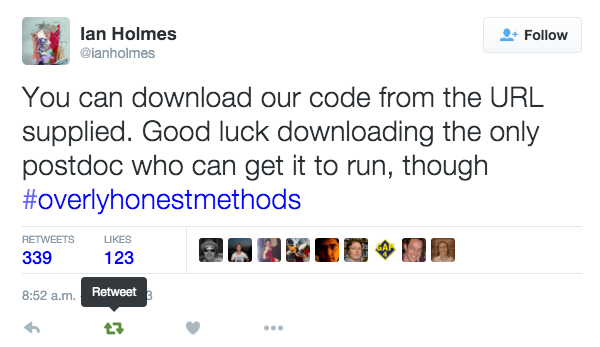
\includegraphics[width=.7\textwidth]{\assetsfolder/please-download-the-postdoc-tweet.png}}
        \end{center}

        % Simply "putting code up" is sadly not a solution. Even though at times
        % it's progress.
    \end{frame}

    \begin{frame}
        \begin{center}
            \href{https://twitter.com/betatim/status/1004077975233552385}{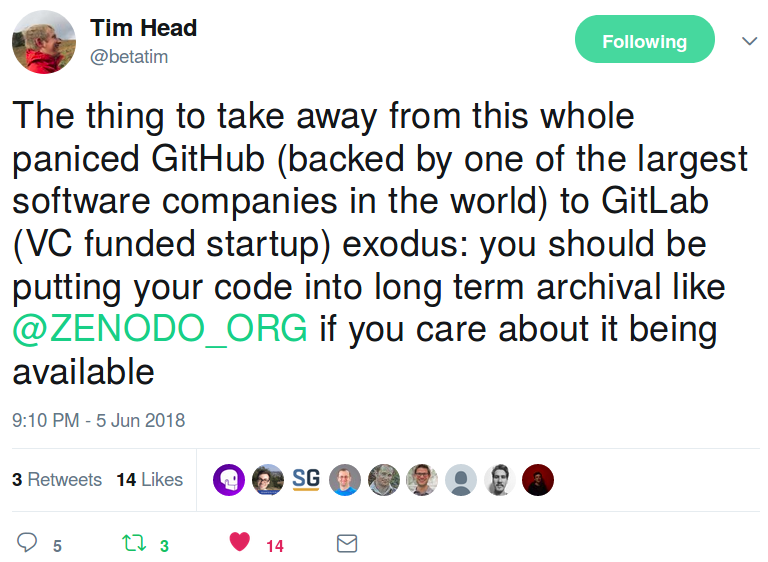
\includegraphics[width=.7\textwidth]{\assetsfolder/ms-github-importance-of-archiving-tweet.png}}
        \end{center}
        % The recent MS + Github saw a number of hot takes. This one in
        % particular I thought was quite good. The problem associated with "just
        % putting your code up" isn't as simple as being able to run it and/or
        % understand it. There are fundamental problems associated to making
        % sure that software is actually there! And that it was/is the software
        % that was actually used to do the research.
    \end{frame}

    \begin{frame}
        \begin{center}
            \href{https://twitter.com/JamesCampbell95/status/996419422951825410}{
\includegraphics[width=.7\textwidth]{\assetsfolder/blockchain-instead-of-archiving-tweet.png}}
        \end{center}

        % There are some great technological solutions: this tweet from a PhD
        % student at Cardiff is 1/4 describing a paper that uses blockhain to
        % ensure archival of all materials.
    \end{frame}

    \begin{frame}
        \begin{center}
            \href{https://twitter.com/legogradstudent/status/979776951517876225}{
\includegraphics[width=.7\textwidth]{\assetsfolder/just-use-git-tweet.png}}
        \end{center}

        % This is a slightly worse to this: tooling is not the only solution
        % (to be clear: this is not a blockchain talk)
        % Just telling people to use tools is not sufficient.
    \end{frame}

	\begin{frame}
		\begin{center}
			\begin{tikzpicture}

				\node [font=\large, draw] (technology) at (-4, 4.5) {Technology};
				\node [font=\large, draw] (culture) at (4, 3.5) {Culture};

				\draw [very thick] (0, 0) -- (0, 6);
				\draw [very thick] (-2, 0) -- (2, 0);

				\draw [very thick] (-4, 6.5) -- (4, 5.5);
				\draw [very thick] (-4, 6.5) -- (technology);
				\draw [very thick] (4, 5.5)  -- (culture);
			\end{tikzpicture}
		\end{center}

        % We need to talk about balancing technology with culture. There are a
        % number of things happening in that sense.
	\end{frame}

	\begin{frame}
	   \begin{center}
		   
\includegraphics[height=6cm]{\assetsfolder/ssi-logo.png}

			\url{https://www.software.ac.uk/}
	   \end{center}

       % The Sustainable Software Institute, is an organisation in the UK that
       % is funded by one of the main research funders and aims to promote
       % better practice in research.

       % One of the many things they do is run a fellowship programme: every
       % year a number of individuals are selected (in quite a competitive
       % environment) to be (lifelong) fellows with goals to spread best
       % practice. For example a PhD student of mine is using his fellowship to
       % give talks and produce learning resources in Welsh (Wales is a bi
       % lingual country).

       % As well as this, the SSI, run a yearly workshop (an unconference) which
       % brings together people from a number of academic fields to discuss and
       % improve the landscape of software in research.
       % Some examples that directly come out of this workshop include `recipy`
       % a Python library that automatically builds up a database of what code
       % ran to produce every output.
	\end{frame}

	\begin{frame}
	   \begin{center}
		   
\includegraphics[height=7cm]{\assetsfolder/UKRSE-logo.png}

			\url{http://rse.ac.uk/}
	   \end{center}

       % Another output is the notion of a research software engineer. They're
       % adamant that anyone who write code and does research is an rse but
       % we're seeing a number of groups arise around the world: with scientists
       % whose role it is to contribute (through writing of software) to the
       % research being done.
    \end{frame}

	\begin{frame}
	   \begin{center}
		   
\includegraphics[width=8cm]{\assetsfolder/the-carpentries-logo.pdf}

			\url{https://carpentries.org/}
	   \end{center}

       % The problem is of course subtle, some of you might have heard of
       % Software carpentry. The carpentries encompasses that as well as what
       % was called the library carpentries. These are a collection of workshops
       % that aim to introduce researchers to the why and how of best practice.
	\end{frame}

	\begin{frame}
	   \begin{center}
           
\includegraphics[width=6cm]{\assetsfolder/joss-logo.png}

			\url{http://joss.theoj.org/}
	   \end{center}

       % We have to ask ourselves what is one of the main reasons for poor
       % practice. I believe, in part because it's good enough. Most
       % promotion/tenure like procedures do not (YET) recognise software.
       % There is ongoing work to recognise software as a research contribution.
       % For example JOSS: a completely open journal. These are short papers
       % that, usually if a piece of code has been written correctly (tested,
       % documented, etc), take very little effort to write.
	\end{frame}

	\begin{frame}
		\Huge
		\begin{center}
			\textit {For example...}
		\end{center}

        % I'm going to give an example of some of the things I've spoken about
        % here.
	\end{frame}

	\begin{frame}
		\begin{center}
			
\includegraphics[width=.7\textwidth]{\assetsfolder/lizard-tweet.png}
		\end{center}
		\begin{center}
			\pause
			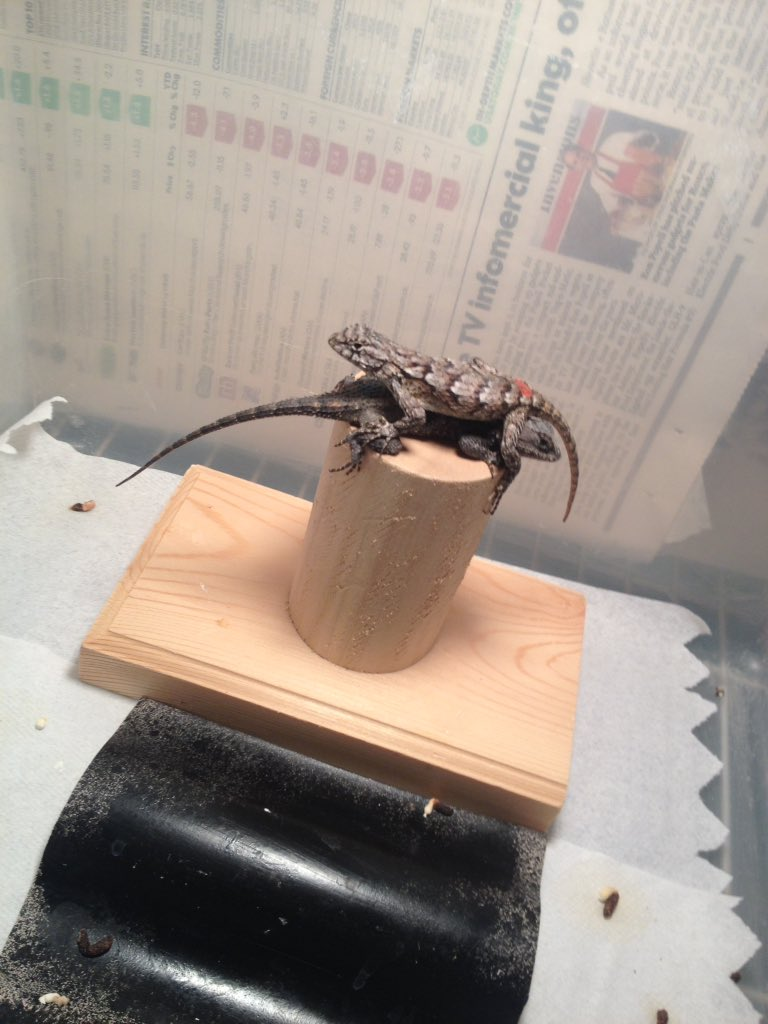
\includegraphics[width=.35\textwidth]
			{\assetsfolder/lizard-cooperation.jpg}
		\end{center}

        % This is a tweet I specifically liked. The idea going on here (I
        % believe), is that we want to study if a specific Lizard is going to
        % dominate another. Perhaps this gets correlated to some genetic marker
        % or even prior behaviour.

        % The reason I like this tweet, is that it is a nice illustration of
        % game theory. Game theory is the study of outcomes based on behaviour
        % in rule based systems. So for example: the lizard that was not fed is
        % more likely to fight and win the warm part of the coop perhaps?

        % [CLICK] Here is the output

        % And the reason this tweet is cool is because it evidences the need for
        % the subject: sometimes out of simple systems we do not get the
        % behaviour we expect. Indeed, here cooperative behaviour has emerged.

	\end{frame}

	\begin{frame}
		\fontsize{74}{65}\selectfont
		\begin{center}
			\(
				\begin{pmatrix}
					3 & 0\\
					5 & 1
				\end{pmatrix}
			\)
		\end{center}

        % A well used game (set of rules) is the Prisoners Dilemma. You might
        % have heard of this game before, the general concept is that you have
        % the option to cooperate or defect when encountering someone else.
        % Cooperation is essentially the selfish action: giving a bit to ensure
        % the individual you encounter gains more. Defection on the other hand
        % is the selfish action: take whatever you can.
        % When both cooperate it's good for both (for example the lizards).
	\end{frame}

	\begin{frame}[fragile]{}
		\begin{columns}
			\begin{column}{.4\textwidth}
				\begin{center}
					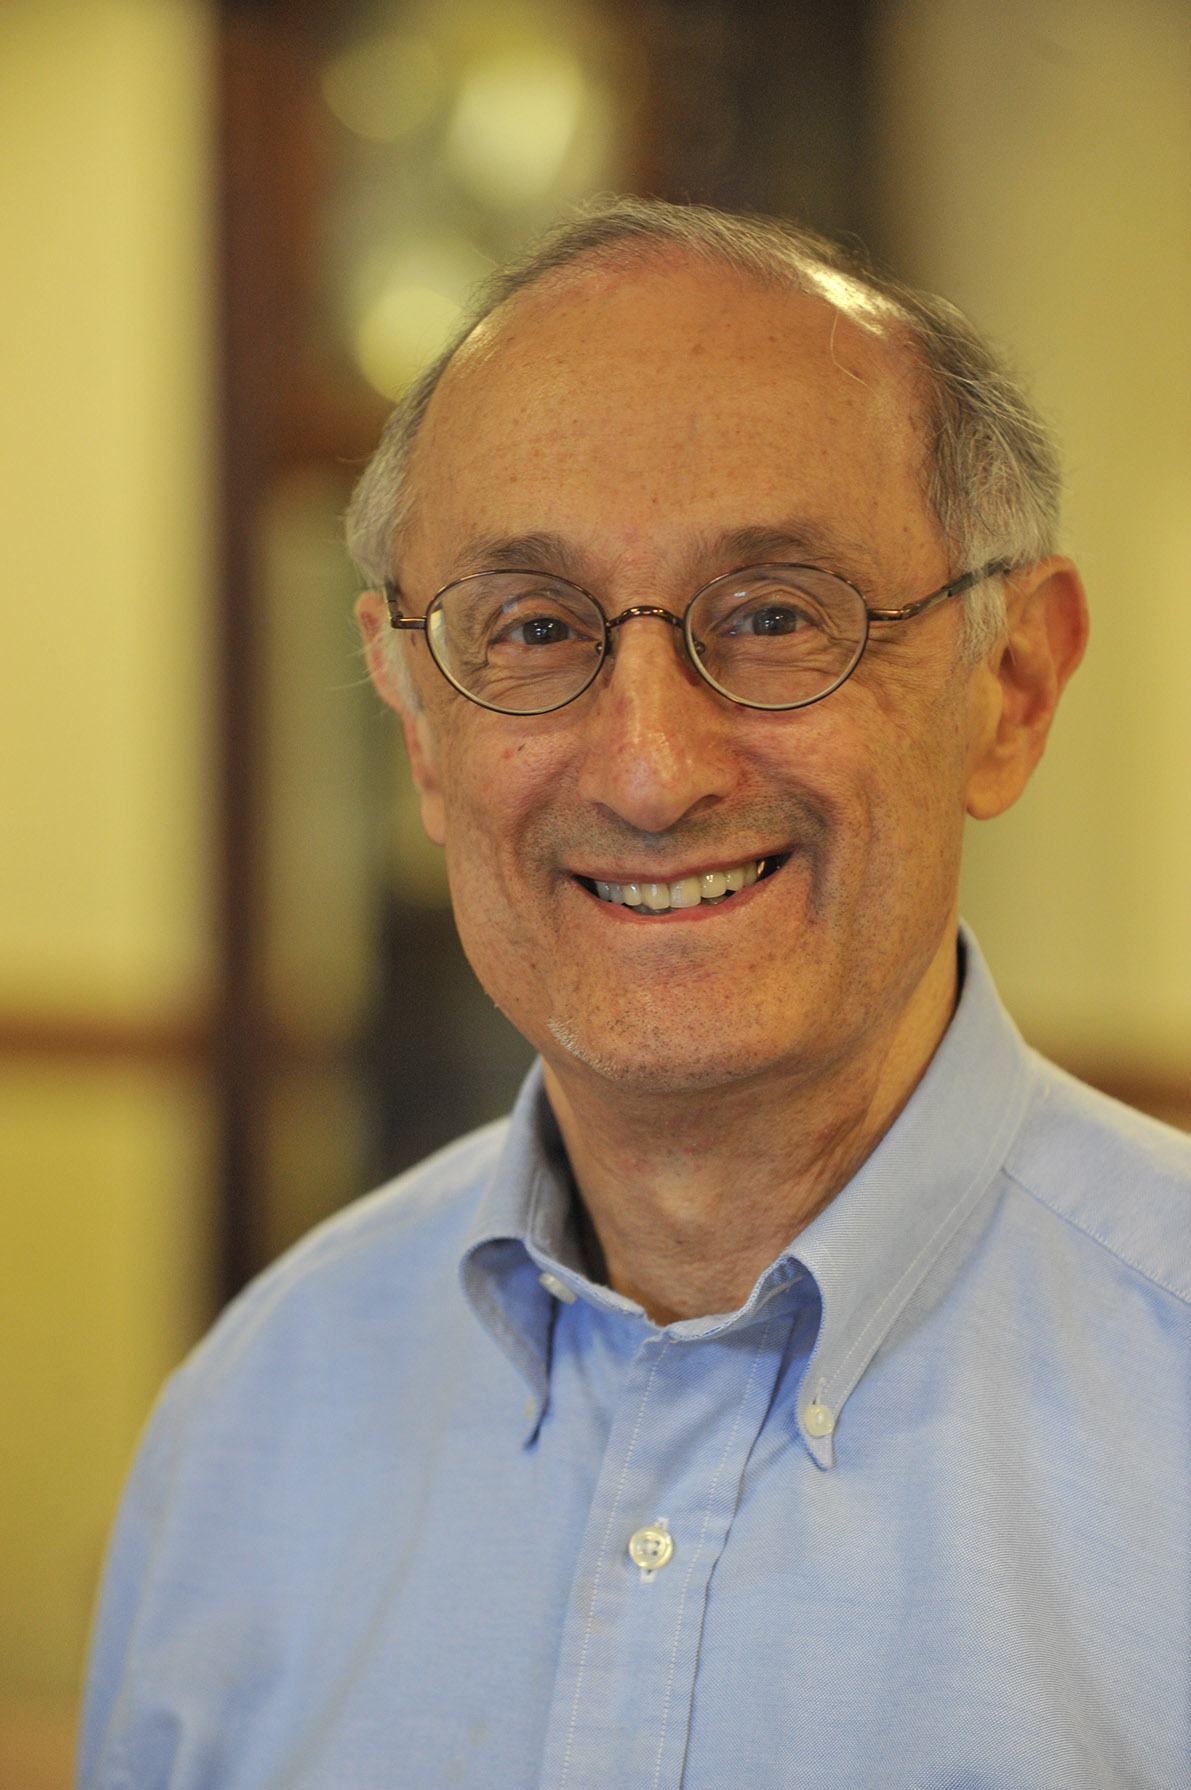
\includegraphics[width=.8\textwidth]{\assetsfolder/Axelrod.jpg}
					\\
					Robert Axelrod
				\end{center}
			\end{column}
			\pause
			\begin{column}{.6\textwidth}
				\begin{minted}[fontsize=\scriptsize]{python}
>>> import axelrod as axl

>>> players = (axl.TitForTat(),
...            axl.Cooperator())
>>> axl.Match(players, turns=5).play()
[(C, C), (C, C), (C, C), (C, C), (C, C)]

>>> players = (axl.TitForTat(),
...            axl.Defector())
>>> axl.Match(players, turns=5).play()
[(C, D), (D, D), (D, D), (D, D), (D, D)]

>>> players = (axl.TitForTat(),
...            axl.Alternator())
>>> axl.Match(players, turns=5).play()
[(C, C), (C, D), (D, C), (C, D), (D, C)]

				\end{minted}
			\end{column}
		\end{columns}

        % A lot of work was done on this subject, dating back to a tournament
        % by Robert Axelrod. He invited individuals to submit code that played
        % this tournament. 1 specific strategy came out on top: TfT.

        % [CLICK]

        % You can see some examples here, this is using a Python library
        % Axelrod. The library allows us to run tournaments, Moran processes and
        % a number of other things.
\end{frame}

    \begin{frame}
        \begin{center}
            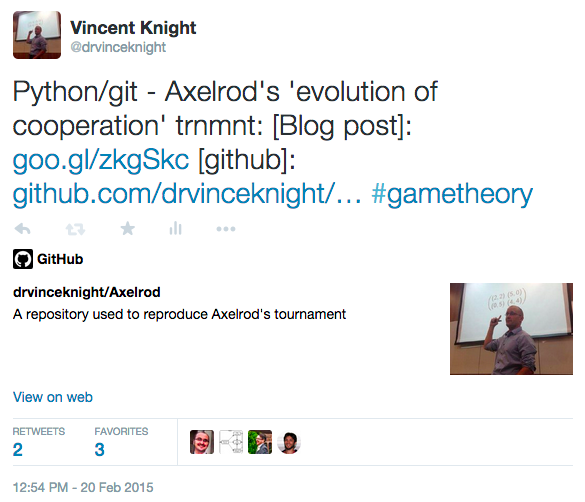
\includegraphics[width=.7\textwidth]{\assetsfolder/axelrod-tweet.png}
        \end{center}

        % This was when the library was announced. A small little tweet and
        % (quite a popular post on G+ actually) that amongst other things
        % brought quite a few contributors. At present the library has 200
        % stars on github.
    \end{frame}

    \begin{frame}
        \begin{center}
            \fontsize{60}{70}\selectfont \(59\)
        \end{center}
    \end{frame}

\begin{frame}[fragile]{}
    \begin{minted}{fortran}
      FUNCTION K92R(J,M,K,L,R, JA)
    C BY ANATOL RAPOPORT
    C TYPED BY AX 3/27/79 (SAME AS ROUND ONE TIT FOR TAT)
    c replaced by actual code, Ax 7/27/93
    c  T=0
    c   K92R=ITFTR(J,M,K,L,T,R)
      k92r=0
      k92r = j
    c test 7/30
    c   write(6,77) j, k92r
    c77   format(' test k92r. j,k92r: ', 2i3)
      RETURN
      END
        \end{minted}

        % Here is what some of the original code: this is Tit For Tat. Written
        % in Fortran.
\end{frame}

\begin{frame}[fragile]{}

    \begin{center}
        \begin{minipage}{0.8\textwidth}
            \begin{minted}[fontsize=\Huge]{python}
import axelrod_fortran
            \end{minted}
        \end{minipage}
    \end{center}

    % One of the liraries in the project is a Python library that wraps the
    % original code. Contributions are regularly coming in that implement these
    % strategies in Python but the wrapper, first of all allows us to check that
    % they are correct and secondly really allows us to run Robert Axelrod's
    % original tournaments!
\end{frame}

    \begin{frame}
        \begin{center}
            \includegraphics[width=.9\textwidth]{\revisitresearchfolder/assets/original_tournament_rankings_all_approaches.pdf}
        \end{center}

        % But even with the code: it is difficult to reproduce the work. This is
        % a number of different ways of computing the results and they do not
        % all match. There could be a number of reasons for this, slightly
        % different compilers: not the EXACT same code. The main conclusions
        % though: do match up. The simple strategy Tit For Tat wins.
    \end{frame}

    \begin{frame}
        \begin{center}
            \includegraphics[width=.9\textwidth]{\revisitresearchfolder/assets/original_tournament_with_extra_strategy_ranks_vs_library_ranks.pdf}
        \end{center}

        % The library has had a number of strategies contributed. We can
        % investigate if one would have changed the results and impressively:
        % no! Tit For Tat still wins.
    \end{frame}

    \begin{frame}
        \begin{center}
            \includegraphics[width=.7\textwidth]{\revisitresearchfolder/assets/full_tournament_pairwise_cooperation_rates.pdf}
        \end{center}

        % However if we run a tournament with all available strategies (the size
        % is too big here) then Tit for Tat no longer wins. The tournament is
        % won by much more complex strategies and what this plot shows here is,
        % is that they all cooperate with each other and/or don't with the lower
        % ranking strategies.
    \end{frame}


    \begin{frame}
        \scalebox{.7}{
            \input{\mlresearchfolder/assets/fsm.tex}
        }

        % One such strategy looks like this: it is called a finite state machine
        % It's just a simple mathematical structure and structures can be
        % trained.
    \end{frame}

\begin{frame}[fragile]{}

    \begin{center}
        \begin{minipage}{0.8\textwidth}
            \begin{minted}[fontsize=\Huge]{python}
import axelrod_dojo
            \end{minted}
        \end{minipage}
    \end{center}

    % Here's another sub project: it's built to allow for training of strategies
    % with reinforcement learning. A number of algorithms are available and in
    % particular they allow us to train structured strategies of the above type
    % by getting them to play in specific environments and then self improve.
\end{frame}


    \begin{frame}
        \begin{center}
            \scalebox{.7}{
                    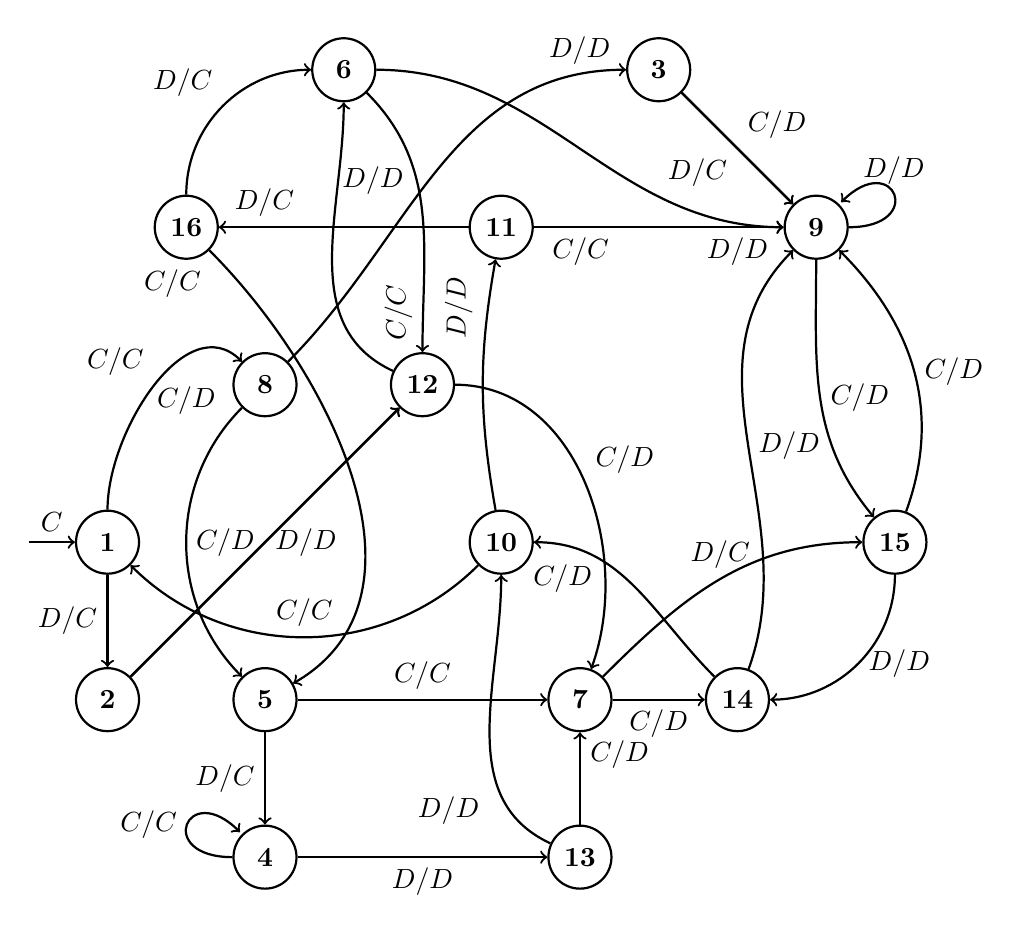
\begin{tikzpicture}

    \tikzstyle{state}=[minimum width=0.8cm, font=\boldmath];
    \node[circle, draw=black, thick] (5) at (0, 0) [state] {$6$};
	\node[circle, draw=black, thick] (2) at (4, 0) [state] {$3$};
	\node[circle, draw=black, thick] (15) at (-2, -2) [state] {$16$};
	\node[circle, draw=black, thick] (8) at ($(2)+(2,-2)$) [state] {$9$};
	\node[circle, draw=black, thick] (10) at ($(15)+(4, 0)$) [state] {$11$};
	
	\node[circle, draw=black, thick] (7) at ($(5)+(-1,-4)$) [state] {$8$};
	\node[circle, draw=black, thick] (11) at ($(7)+(2, 0)$) [state] {$12$};



	\node[circle, draw=black, thick] (9) at ($(10)+(0,-4)$) [state] {$10$};
	\node[circle, draw=black, thick] (0) at ($(9)+(-5,0)$) [state] {$1$};
	\node[circle, draw=black, thick] (14) at ($(9)+(5,0)$) [state] {$15$};

	\node[circle, draw=black, thick] (1) at ($(0)+(0,-2)$) [state] {$2$};
	\node[circle, draw=black, thick] (4) at ($(1)+(2,0)$) [state] {$5$};
	\node[circle, draw=black, thick] (6) at ($(4)+(4,0)$) [state] {$7$};
	\node[circle, draw=black, thick] (13) at ($(6)+(2,0)$) [state] {$14$};

	\node[circle, draw=black, thick] (3) at ($(4)+(0,-2)$) [state] {$4$};
	\node[circle, draw=black, thick] (12) at ($(6)+(0,-2)$) [state] {$13$};


    \coordinate[left of=0] (s);

    \draw (s) edge[out=0, in=180, ->, thick] node [above] {$C$} (0);
    \draw (0) edge[out=90, in=135, ->, thick] node [above left] {$C/C$} (7);
    \draw (0) edge[out=-90, in=90, ->, thick] node [left] {$D/C$} (1);

    \draw (1) edge[out=45, in=-135, ->, thick] node [left] {$C/D$} (11);
    \draw (1) edge[out=45, in=-135, ->, thick] node [right] {$D/D$} (11);
    
    \draw (2) edge[out=-45, in=135, ->, thick] node [above right] {$C/D$} (8);
    \draw (2) edge[out=-45, in=135, ->, thick] node [below left] {$D/C$} (8);

    \draw (3) edge[out=180, in=135, ->, thick, loop] node [left] {$C/C$} (3);
    \draw (3) edge[out=0, in=180, ->, thick] node [below] {$D/D$} (12);

    \draw (4) edge[out=0, in=180, ->, thick] node [above] {$C/C$} (6);
    \draw (4) edge[out=-90, in=90, ->, thick] node [left] {$D/C$} (3);

    \draw (5) edge[out=0, in=180, ->, thick] node [below, yshift=-1cm, xshift=2cm] {$D/D$} (8);
    \draw (5) edge[out=-45, in=90, ->, thick] node [left, yshift=-0.8cm, xshift=-0.3cm, rotate=90] {$C/C$} (11);

    \draw (6) edge[out=0, in=180, ->, thick] node [below] {$C/D$} (13);
    \draw (6) edge[out=45, in=180, ->, thick] node [above] {$D/C$} (14);

    \draw (7) edge[out=-135, in=135, ->, thick] node [yshift=1.8cm] {$C/D$} (4);
    \draw (7) edge[out=45, in=180, ->, thick] node [above, yshift=1.2cm, xshift=1.8cm] {$D/D$} (2);

    \draw (8) edge[out=0, in=45, ->, thick, loop] node [above] {$D/D$} (8);
    \draw (8) edge[out=-90, in=130, ->, thick] node [right] {$C/D$} (14);

    \draw (9) edge[out=-135, in=-45, ->, thick] node [above] {$C/C$} (0);
    \draw (9) edge[out=100, in=-100, ->, thick] node [above left, yshift=1.5cm, rotate=90] {$D/D$} (10);

    \draw (10) edge[out=0, in=180, ->, thick] node [below left, xshift=-0.5cm] {$C/C$} (8);
    \draw (10) edge[out=180, in=0, ->, thick] node [above left, xshift=-0.5cm] {$D/C$} (15);

    \draw (11) edge[out=0, in=70, ->, thick] node [above right] {$C/D$} (6);
    \draw (11) edge[out=155, in=-90, ->, thick] node [right, yshift=1cm] {$D/D$} (5);

    \draw (12) edge[out=90, in=-90, ->, thick] node [above right] {$C/D$} (6);
    \draw (12) edge[out=155, in=-90, ->, thick] node [left, yshift=-1cm] {$D/D$} (9);

    \draw (13) edge[out=135, in=0, ->, thick] node [below left, xshift=-0.4cm, yshift=0.4cm] {$C/D$} (9);
    \draw (13) edge[out=70, in=-135, ->, thick] node [right] {$D/D$} (8);

    \draw (14) edge[out=70, in=-45, ->, thick] node [right] {$C/D$} (8);
    \draw (14) edge[out=-90, in=0, ->, thick] node [right] {$D/D$} (13);

    \draw (15) edge[out=-45, in=30, ->, thick] node [left, xshift=-1.8cm, yshift=2.5cm] {$C/C$} (4);
    \draw (15) edge[out=90, in=180, ->, thick] node [above left] {$D/C$} (5);

    \end{tikzpicture}

            }
        \end{center}

        % This is a particular such strategy. It's actually trained for
        % something a bit more specific than a tournament but to actually
        % survive in an evolutionary context. The process chose is called a
        % Moran process. Individual bump in to each other and play.
    \end{frame}


    \begin{frame}
        \begin{center}
            
\includegraphics[height=.8\textheight]{./assets/hunger-games-hand-gesture.eps}


            \tiny
            \vfill
            \flushright{Image made by \url{http://www.freepik.com} from
            \url{https://www.flaticon.com} is licensed by CC BY 3.0}
        \end{center}

        % A piece of work that we have doe is to essentially carry out Axelrod's
        % tournament but instead of matches: use Moran process. This allows us
        % to investigate strategies/behaviour that would either be good at
        % resisting change or causing change.
    \end{frame}


    \begin{frame}
        \scriptsize
        \begin{center}
            \textbf{Invasion (\(N=14\))}\\

            \input{\moranresearchfolder/tex/summary_top_14_invade.tex}
        \end{center}

        % Here is the strategies that were best suited to invading groups of
        % others. We see that all the ones that do well are ones that have been
        % trained.
    \end{frame}

    \begin{frame}
        \scriptsize
        \begin{center}
            \textbf{Resistance (\(N=14\))}\\

            \input{\moranresearchfolder/tex/summary_top_14_resist.tex}
        \end{center}

        % Here are the resistors. Again, you that TF* (which stands for trained
        % finite) do well. These are strategies that are specifically trained in
        % Moran environments (the previous ones were just trained to score
        % highly against opponents).
    \end{frame}

    \begin{frame}
        \begin{columns}
            \begin{column}{.6\textwidth}
                \begin{center}
                    \scalebox{.49}{
                            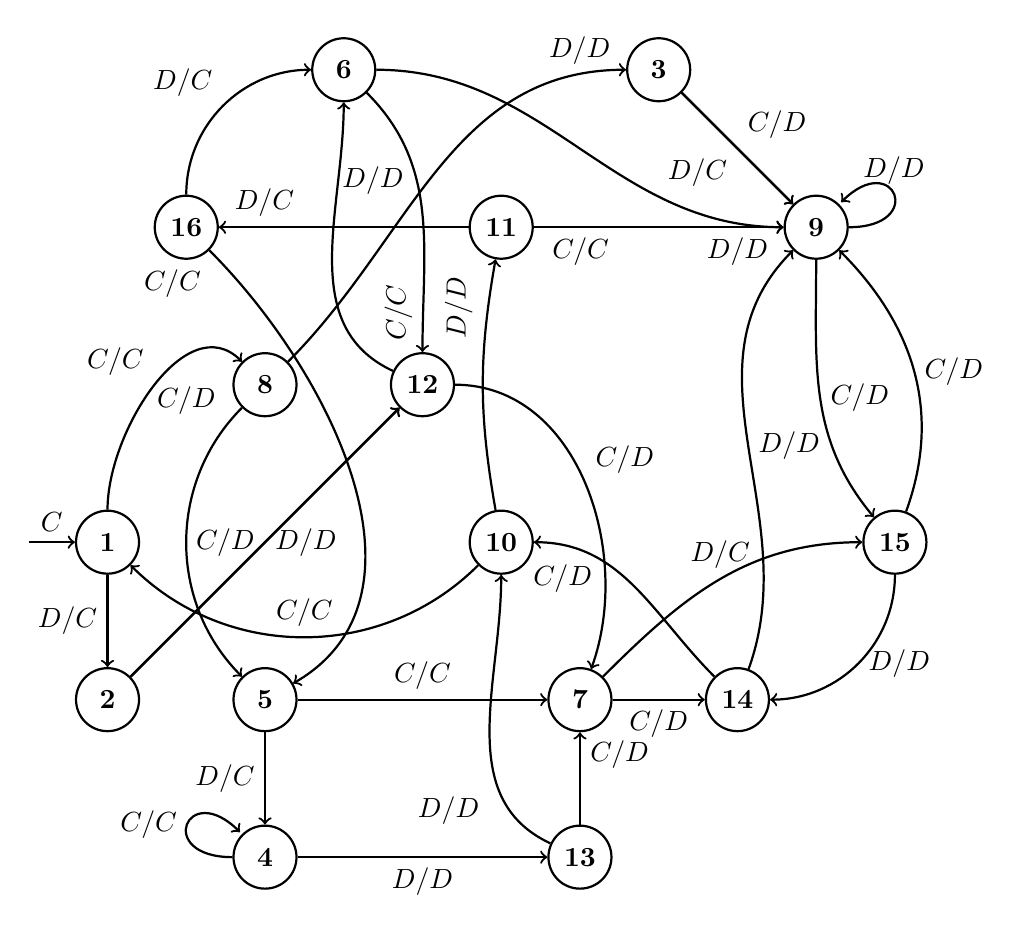
\begin{tikzpicture}

    \tikzstyle{state}=[minimum width=0.8cm, font=\boldmath];
    \node[circle, draw=black, thick] (5) at (0, 0) [state] {$6$};
	\node[circle, draw=black, thick] (2) at (4, 0) [state] {$3$};
	\node[circle, draw=black, thick] (15) at (-2, -2) [state] {$16$};
	\node[circle, draw=black, thick] (8) at ($(2)+(2,-2)$) [state] {$9$};
	\node[circle, draw=black, thick] (10) at ($(15)+(4, 0)$) [state] {$11$};
	
	\node[circle, draw=black, thick] (7) at ($(5)+(-1,-4)$) [state] {$8$};
	\node[circle, draw=black, thick] (11) at ($(7)+(2, 0)$) [state] {$12$};



	\node[circle, draw=black, thick] (9) at ($(10)+(0,-4)$) [state] {$10$};
	\node[circle, draw=black, thick] (0) at ($(9)+(-5,0)$) [state] {$1$};
	\node[circle, draw=black, thick] (14) at ($(9)+(5,0)$) [state] {$15$};

	\node[circle, draw=black, thick] (1) at ($(0)+(0,-2)$) [state] {$2$};
	\node[circle, draw=black, thick] (4) at ($(1)+(2,0)$) [state] {$5$};
	\node[circle, draw=black, thick] (6) at ($(4)+(4,0)$) [state] {$7$};
	\node[circle, draw=black, thick] (13) at ($(6)+(2,0)$) [state] {$14$};

	\node[circle, draw=black, thick] (3) at ($(4)+(0,-2)$) [state] {$4$};
	\node[circle, draw=black, thick] (12) at ($(6)+(0,-2)$) [state] {$13$};


    \coordinate[left of=0] (s);

    \draw (s) edge[out=0, in=180, ->, thick] node [above] {$C$} (0);
    \draw (0) edge[out=90, in=135, ->, thick] node [above left] {$C/C$} (7);
    \draw (0) edge[out=-90, in=90, ->, thick] node [left] {$D/C$} (1);

    \draw (1) edge[out=45, in=-135, ->, thick] node [left] {$C/D$} (11);
    \draw (1) edge[out=45, in=-135, ->, thick] node [right] {$D/D$} (11);
    
    \draw (2) edge[out=-45, in=135, ->, thick] node [above right] {$C/D$} (8);
    \draw (2) edge[out=-45, in=135, ->, thick] node [below left] {$D/C$} (8);

    \draw (3) edge[out=180, in=135, ->, thick, loop] node [left] {$C/C$} (3);
    \draw (3) edge[out=0, in=180, ->, thick] node [below] {$D/D$} (12);

    \draw (4) edge[out=0, in=180, ->, thick] node [above] {$C/C$} (6);
    \draw (4) edge[out=-90, in=90, ->, thick] node [left] {$D/C$} (3);

    \draw (5) edge[out=0, in=180, ->, thick] node [below, yshift=-1cm, xshift=2cm] {$D/D$} (8);
    \draw (5) edge[out=-45, in=90, ->, thick] node [left, yshift=-0.8cm, xshift=-0.3cm, rotate=90] {$C/C$} (11);

    \draw (6) edge[out=0, in=180, ->, thick] node [below] {$C/D$} (13);
    \draw (6) edge[out=45, in=180, ->, thick] node [above] {$D/C$} (14);

    \draw (7) edge[out=-135, in=135, ->, thick] node [yshift=1.8cm] {$C/D$} (4);
    \draw (7) edge[out=45, in=180, ->, thick] node [above, yshift=1.2cm, xshift=1.8cm] {$D/D$} (2);

    \draw (8) edge[out=0, in=45, ->, thick, loop] node [above] {$D/D$} (8);
    \draw (8) edge[out=-90, in=130, ->, thick] node [right] {$C/D$} (14);

    \draw (9) edge[out=-135, in=-45, ->, thick] node [above] {$C/C$} (0);
    \draw (9) edge[out=100, in=-100, ->, thick] node [above left, yshift=1.5cm, rotate=90] {$D/D$} (10);

    \draw (10) edge[out=0, in=180, ->, thick] node [below left, xshift=-0.5cm] {$C/C$} (8);
    \draw (10) edge[out=180, in=0, ->, thick] node [above left, xshift=-0.5cm] {$D/C$} (15);

    \draw (11) edge[out=0, in=70, ->, thick] node [above right] {$C/D$} (6);
    \draw (11) edge[out=155, in=-90, ->, thick] node [right, yshift=1cm] {$D/D$} (5);

    \draw (12) edge[out=90, in=-90, ->, thick] node [above right] {$C/D$} (6);
    \draw (12) edge[out=155, in=-90, ->, thick] node [left, yshift=-1cm] {$D/D$} (9);

    \draw (13) edge[out=135, in=0, ->, thick] node [below left, xshift=-0.4cm, yshift=0.4cm] {$C/D$} (9);
    \draw (13) edge[out=70, in=-135, ->, thick] node [right] {$D/D$} (8);

    \draw (14) edge[out=70, in=-45, ->, thick] node [right] {$C/D$} (8);
    \draw (14) edge[out=-90, in=0, ->, thick] node [right] {$D/D$} (13);

    \draw (15) edge[out=-45, in=30, ->, thick] node [left, xshift=-1.8cm, yshift=2.5cm] {$C/C$} (4);
    \draw (15) edge[out=90, in=180, ->, thick] node [above left] {$D/C$} (5);

    \end{tikzpicture}

                    }
                \end{center}
            \end{column}

            \begin{column}{.4\textwidth}
                \small
                \begin{tabular}{ll}
                    \toprule
                    TF1 \#1   & TF1 \#2\\
                    \midrule
                    \bf{1}: C & \bf{1}: C  \\
                    \bf{8}: C & \bf{8}: C  \\
                    \bf{5}: D & \bf{5}: D  \\
                    4: C      & 4: C  \\
                    4: C      & 4: C  \\
                    4: C      & 4: C  \\
                    4: C      & 4: C  \\
                    4: C      & 4: C  \\
                    \bottomrule
                \end{tabular}
            \end{column}
        \end{columns}

        % Let us take a close look at TF1: when playing against itself we see
        % that it'll have this 3 turn handshake.
        % Importantly this was not trained: this is the output of an
        % evolutionary process.

        % So, going back to Axelrod's original work, we see that TfT was almost
        % certainly not sufficiently sophisticated but one in the simple
        % environment. It has a very naive self recognition mechanism (it in
        % essence self recognises a number of strategies) but what this
        % extension of the work allows us to do is show that it is probably that
        % strong vectors of spread of behaviour are self recognition mechanisms.
    \end{frame}


    \begin{frame}
        \Huge
        \begin{center}
            \only<1>{
                164
                }
            \only<2>{
                \sout{164}\; 213+
                }
        \end{center}

        % This training is only possible because of the very diverse training
        % potential. At the time of doing that work, we had 164 strategies,
        % right now we have had over 200. The really nice thing about this is
        % that this is completely open work and a lot of contributions to the
        % work are not by academics but by a wide diversity of areas.
    \end{frame}


\begin{frame}
    \begin{footnotesize}
        \begin{tcolorbox}[colback=github,colframe=blue!40!black,title=
                Julie Rymer - \href{https://gitter.im/Axelrod-Python/Axelrod?at=591388592b926f8a6741435d}
                {@Chadys} - (10 May 2017):
    ]
                And I really wanted to thank you all, I discovered your project because of a
                course where we needed to participate in an open source project, and I had the
                occasion to compare the welcome me and my coworkers received here compared to
                other people from my class who worked on different project. And I've got to said
                you are awesome on that part and on the help your provide to newbies  I like
                your project so I'll try to continue to contribute now and then !
       \end{tcolorbox}
    \end{footnotesize}

   \begin{columns}
        \begin{column}{.35\textwidth}
            \begin{itemize}
                \item \href{https://twitter.com/NikoletaGlyn}{@NikoletaGlyn}
                \item \href{https://twitter.com/opcampbell}{@opcampbell}
                \item \href{http://marcharper.codes/}{marcharper.codes}
            \end{itemize}
        \end{column}
        \begin{column}{.65\textwidth}
            \begin{itemize}
                \item \href{https://github.com/Axelrod-Python/Axelrod}{github.com/Axelrod-Python/Axelrod}
                \item \href{https://gitter.im/Axelrod-Python/Axelrod}{gitter.im/Axelrod-Python/Axelrod}
                \item
                    \href{https://arxiv.org/abs/1707.06920}{arxiv.org/abs/1707.06920}
            \end{itemize}
        \end{column}
   \end{columns}

        \begin{center}
               \href{https://twitter.com/drvinceknight}{@drvinceknight}
        \end{center}

   \begin{columns}
        \begin{column}{.5\textwidth}
            \begin{itemize}
                \item
                    \href{https://www.software.ac.uk/}{software.ac.uk}
                \item
                    \href{http://rse.ac.uk/}{rse.ac.uk}
            \end{itemize}
        \end{column}
        \begin{column}{.5\textwidth}
            \begin{itemize}
            \item
                \href{https://carpentries.org/}{carpentries.org}
            \item
                \href{http://joss.theoj.org/}{joss.theoj.org}
            \end{itemize}
        \end{column}
    \end{columns}
\end{frame}


\end{document}
